% This file was created with tikzplotlib v0.9.17.
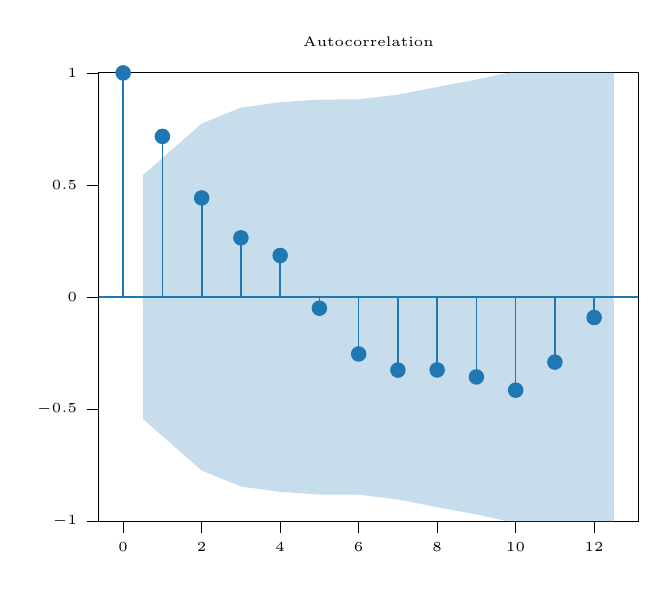
\begin{tikzpicture}

\definecolor{color0}{rgb}{0.12156862745098,0.466666666666667,0.705882352941177}

\begin{axis}[
font={\fontsize{3}{12}\selectfont},
tick align=outside,
tick pos=left,
title={Autocorrelation},
x grid style={white!69.0196078431373!black},
xmin=-0.625, xmax=13.125,
xtick style={color=black},
y grid style={white!69.0196078431373!black},
ymin=-1, ymax=1,
ytick style={color=black}
]
\path [fill=color0, fill opacity=0.25]
(axis cs:0.5,0.543596203409375)
--(axis cs:0.5,-0.543596203409375)
--(axis cs:2,-0.773947598601257)
--(axis cs:3,-0.845276373185772)
--(axis cs:4,-0.869312205352692)
--(axis cs:5,-0.880919874555284)
--(axis cs:6,-0.881752016017819)
--(axis cs:7,-0.90310763168253)
--(axis cs:8,-0.937191082551989)
--(axis cs:9,-0.969976301352679)
--(axis cs:10,-1.00791234083313)
--(axis cs:11,-1.05729910132389)
--(axis cs:12.5,-1.08060211348733)
--(axis cs:12.5,1.08060211348733)
--(axis cs:12.5,1.08060211348733)
--(axis cs:11,1.05729910132389)
--(axis cs:10,1.00791234083313)
--(axis cs:9,0.969976301352679)
--(axis cs:8,0.937191082551989)
--(axis cs:7,0.90310763168253)
--(axis cs:6,0.881752016017819)
--(axis cs:5,0.880919874555284)
--(axis cs:4,0.869312205352692)
--(axis cs:3,0.845276373185772)
--(axis cs:2,0.773947598601257)
--(axis cs:0.5,0.543596203409375)
--cycle;

\path [draw=color0, semithick]
(axis cs:0,0)
--(axis cs:0,1);

\path [draw=color0, semithick]
(axis cs:1,0)
--(axis cs:1,0.716616068448596);

\path [draw=color0, semithick]
(axis cs:2,0)
--(axis cs:2,0.442073448242865);

\path [draw=color0, semithick]
(axis cs:3,0)
--(axis cs:3,0.264069432381399);

\path [draw=color0, semithick]
(axis cs:4,0)
--(axis cs:4,0.185408191893314);

\path [draw=color0, semithick]
(axis cs:5,0)
--(axis cs:5,-0.0498187593112183);

\path [draw=color0, semithick]
(axis cs:6,0)
--(axis cs:6,-0.253960790944796);

\path [draw=color0, semithick]
(axis cs:7,0)
--(axis cs:7,-0.325780082133312);

\path [draw=color0, semithick]
(axis cs:8,0)
--(axis cs:8,-0.325268521742456);

\path [draw=color0, semithick]
(axis cs:9,0)
--(axis cs:9,-0.356316144041773);

\path [draw=color0, semithick]
(axis cs:10,0)
--(axis cs:10,-0.415428338267509);

\path [draw=color0, semithick]
(axis cs:11,0)
--(axis cs:11,-0.290341044762263);

\path [draw=color0, semithick]
(axis cs:12,0)
--(axis cs:12,-0.0912534597628461);

\addplot [semithick, color0]
table {%
-0.625 -2.22044604925031e-16
13.125 -2.22044604925031e-16
};
\addplot [semithick, color0, mark=*, mark size=2.5, mark options={solid}, only marks]
table {%
0 1
1 0.716616068448596
2 0.442073448242865
3 0.264069432381399
4 0.185408191893314
5 -0.0498187593112183
6 -0.253960790944796
7 -0.325780082133312
8 -0.325268521742456
9 -0.356316144041773
10 -0.415428338267509
11 -0.290341044762263
12 -0.0912534597628461
};
\end{axis}

\end{tikzpicture}
